\chapter{Introdução}

\section{Motivação}
Há uma expectativa de que o número de casas inteligentes aumente cerca de 17\% nos Estados Unidos no ano de 2017 \cite{mckinseyReport}, onde já se tem investimentos de grandes empresas, como Google, Amazon e Apple, mostrando a relevância do tema no momento atual. O interesse nessa área é tamanho que a Google investiu cerca de 5 milhões de dólares em um comercial de seu produto Google Home no Super Bowl 2017 (final de futebol americano nos EUA) \cite{kennemer}.

Assim, as oportunidades trazidas pelo conceito de Internet das Coisas (IoT) à área de automação residencial são uma grande motivação para esse projeto. Também destacam-se as possibilidades de promover tais tecnologias de casas inteligentes ao mercado nacional, personalizando produtos e adequando-as às necessidades dos potenciais consumidores brasileiros. Mesmo nos Estados Unidos, ainda é necessário algum tempo até que as casas conectadas se consolidem, de modo que há grandes oportunidade de pioneirismo no mercado brasileiro, com o lançamento de produtos de IoT a preços acessíveis e focando nas necessidades dos consumidores locais.

\section{Projeto Hedwig}

\subsection{Objetivo}
A contribuição do projeto será um sistema baseado em arquitetura local modularizada, e em camadas, com funcionalidades local e em nuvem, e provedor de uma \textit{API} que permita seu acesso por diversos clientes - como \textit{websites} ou aplicativos para \textit{smartphones} - que seja capaz de monitorar e agir em diversos módulos presentes na residência do usuário final do sistema. O projeto irá disponibilizar módulos físicos, prontos para serem instalados e configurados na residência, sem que seja necessário conhecimentos avançados de eletrônica ou computação.

Desta forma, os principais pontos do projeto são:

\begin{itemize}
\item \textbf{Robustez}

3 níveis de funcionamento: Online, Local e Offline, para garantir a disponibilidade mesmo com problemas (queda do servidor, internet indisponível, falha no roteador), com medidas para a tentativa automática de reconexão, monitoramento e manutenções preventivas e corretivas do sistema.

\item \textbf{Modularidade}

Garante a independência de funcionamento dos módulos que atendem às várias necessidades, contribuindo para a robustez. Diminui o custo e personaliza o produto, de acordo com as necessidades do cliente.

\item \textbf{Camadas}

O funcionamento da aplicação decorre em diversos níveis e camadas, de responsabilidades independentes, permitindo maior separação de responsabilidades.

\item \textbf{Machine Learning}

Levantamento de rotinas para gerar conhecimento, que se mostra como notificações, alertas e acionamentos automáticos de funções para o cliente.

\item \textbf{Segurança}

Utilização de criptografia assimétrica para comunicação entre servidor local e serviços de nuvem, juntamente com conexão por \textit{WebSocket}. Autenticação e autorização de usuários por métodos \textit{WebToken}. Uso de canais \textit{Publisher/Subscriber} protegidos para troca de mensagens.

\end{itemize}

\subsection{Nome do Projeto}
O nome do projeto foi escolhido em homenagem a Hedy Lamarr. Nascida Hedwig Eva Maria Kiesler \cite{shearer}, a atriz e inventora desenvolveu, durante a Segunda Guerra Mundial, um aparelho de interferência em rádio para despistar radares nazistas, cujos princípios estão incorporados nas tecnologias atuais de Wi-fi, CDMA e Bluetooth \cite{electronicFrontier}. Baseado na ideia de um sistema de comunicação seguro, e como reconhecimento de seu trabalho, foi dado esse nome ao projeto aqui descrito.

\subsection{Logo}
O logo do projeto é uma coruja, também em referência à coruja \textit{Hedwig}, pertencente ao personagem \textit{Harry Potter}, da série de livros de mesmo nome.
\begin{figure}[H]
	\centering
	\caption{Projeto Hedwig}
  
\includegraphics[width=0.2\textwidth]{hedwigLogo}
\label{fig:hedwigLogo}
\end{figure}

\section{Aplicações}
Como aplicações do projeto Hedwig, destacam-se a automação no uso de eletrodomésticos e iluminação, segurança no acesso à casa, economia nas contas de água e energia elétrica, além de um monitoramento remoto de pessoas que moram sozinhas (como é o caso de idosos), garantindo a tranquilidade de seus familiares e mantendo a segurança do indivíduo.

Exemplos de módulos que podem ser incluídos no sistema são: quarto (despertador, iluminação, monitoramento de temperatura e umidade); cozinha (\textit{timer}, iluminação, monitoramento de presença e gás); acesso (controle de abertura, monitoramento de estado); externo (monitoramento de temperatura, umidade, energia elétrica e consumo de água); corredor (monitoramento de presença, iluminação), chuveiro (controle de temperatura\slash potência a partir do perfil de usuário e temperatura externa) e ar condicionado (controle da potência a partir do monitoramento das temperaturas internas e externas da casa).

\subsection{Aplicações de Machine Learning}
\textbf{REVISAR TODA ESSA PARTE}\\
Como possíveis perguntas a serem respondidas pelo módulo de Machine Learning do projeto e os dados a serem coletados (em diferentes lugares da casa), temos:

\begin{itemize}
	
\item Quando notificar a chegada de pessoas ou ambiente vazio? - presença e sensor de abertura do portão
\item Quando enviar alertas de atividade suspeita? - presença
\item Quanto o sistema é usado? (Por funcionalidade) - sensor de abertura e log de aberturas pelo módulo
\item Quando notificar condições insalubres, como temperatura e umidade altas persistentes? - temperatura e umidade
\item Quando notificar falta de atividades rotineiras (como acordar, almoçar) - presença
\item Melhor horário para despertar? - presença
\item Notificar mudança brusca de temperatura, principalmente esfriamento? - temperaturas interna e externa, umidade (para sensação térmica)
\item Quanto o sistema está indisponível na instalação do cliente? - log de qualquer dado periódico
\item Quando acender ou apagar a luz? - presença, acionamento manual (horário e módulo)
\item Quantas vezes notificar? Prioridades? - respostas do cliente (log), para notificar o mínimo necessário, e classificação de notificações (email, somente quando usuário abre o aplicativo, notificação no celular e até módulo de painel externo com buzzer, no caso de comunicação de situação de perigo entre residências fisicamente separadas).
\end{itemize}

Respondendo a essas perguntas, esperamos contribuir para a construção de um sistema autônomo, que aprende com feedbacks do usuário seja pelo monitoramento por módulos ou respostas dadas pelo aplicativo, atuando em segurança (safety), saúde e A
automação da residência do cliente.

\subsection{Módulo de Acesso}

\textbf{Essa definição não deve estar na introdução. Mudar para onde fizer sentido}

Buscando garantir mais segurança e comodidade para o acesso à residência, além dO controle de abertura, o módulo de acesso atua em paralelo com uma fechadura eletrônica, que é acionada por meio do controle, que utiliza ondas de rádio. Assim, mesmo com falha total do sistema, o usuário pode abrir o portão diretamente, sem a necessidade de acesso à internet.

\begin{figure}[H]
	\centering
	\caption{Diagrama ilustrativo do módulo de Acesso ao Portão}
  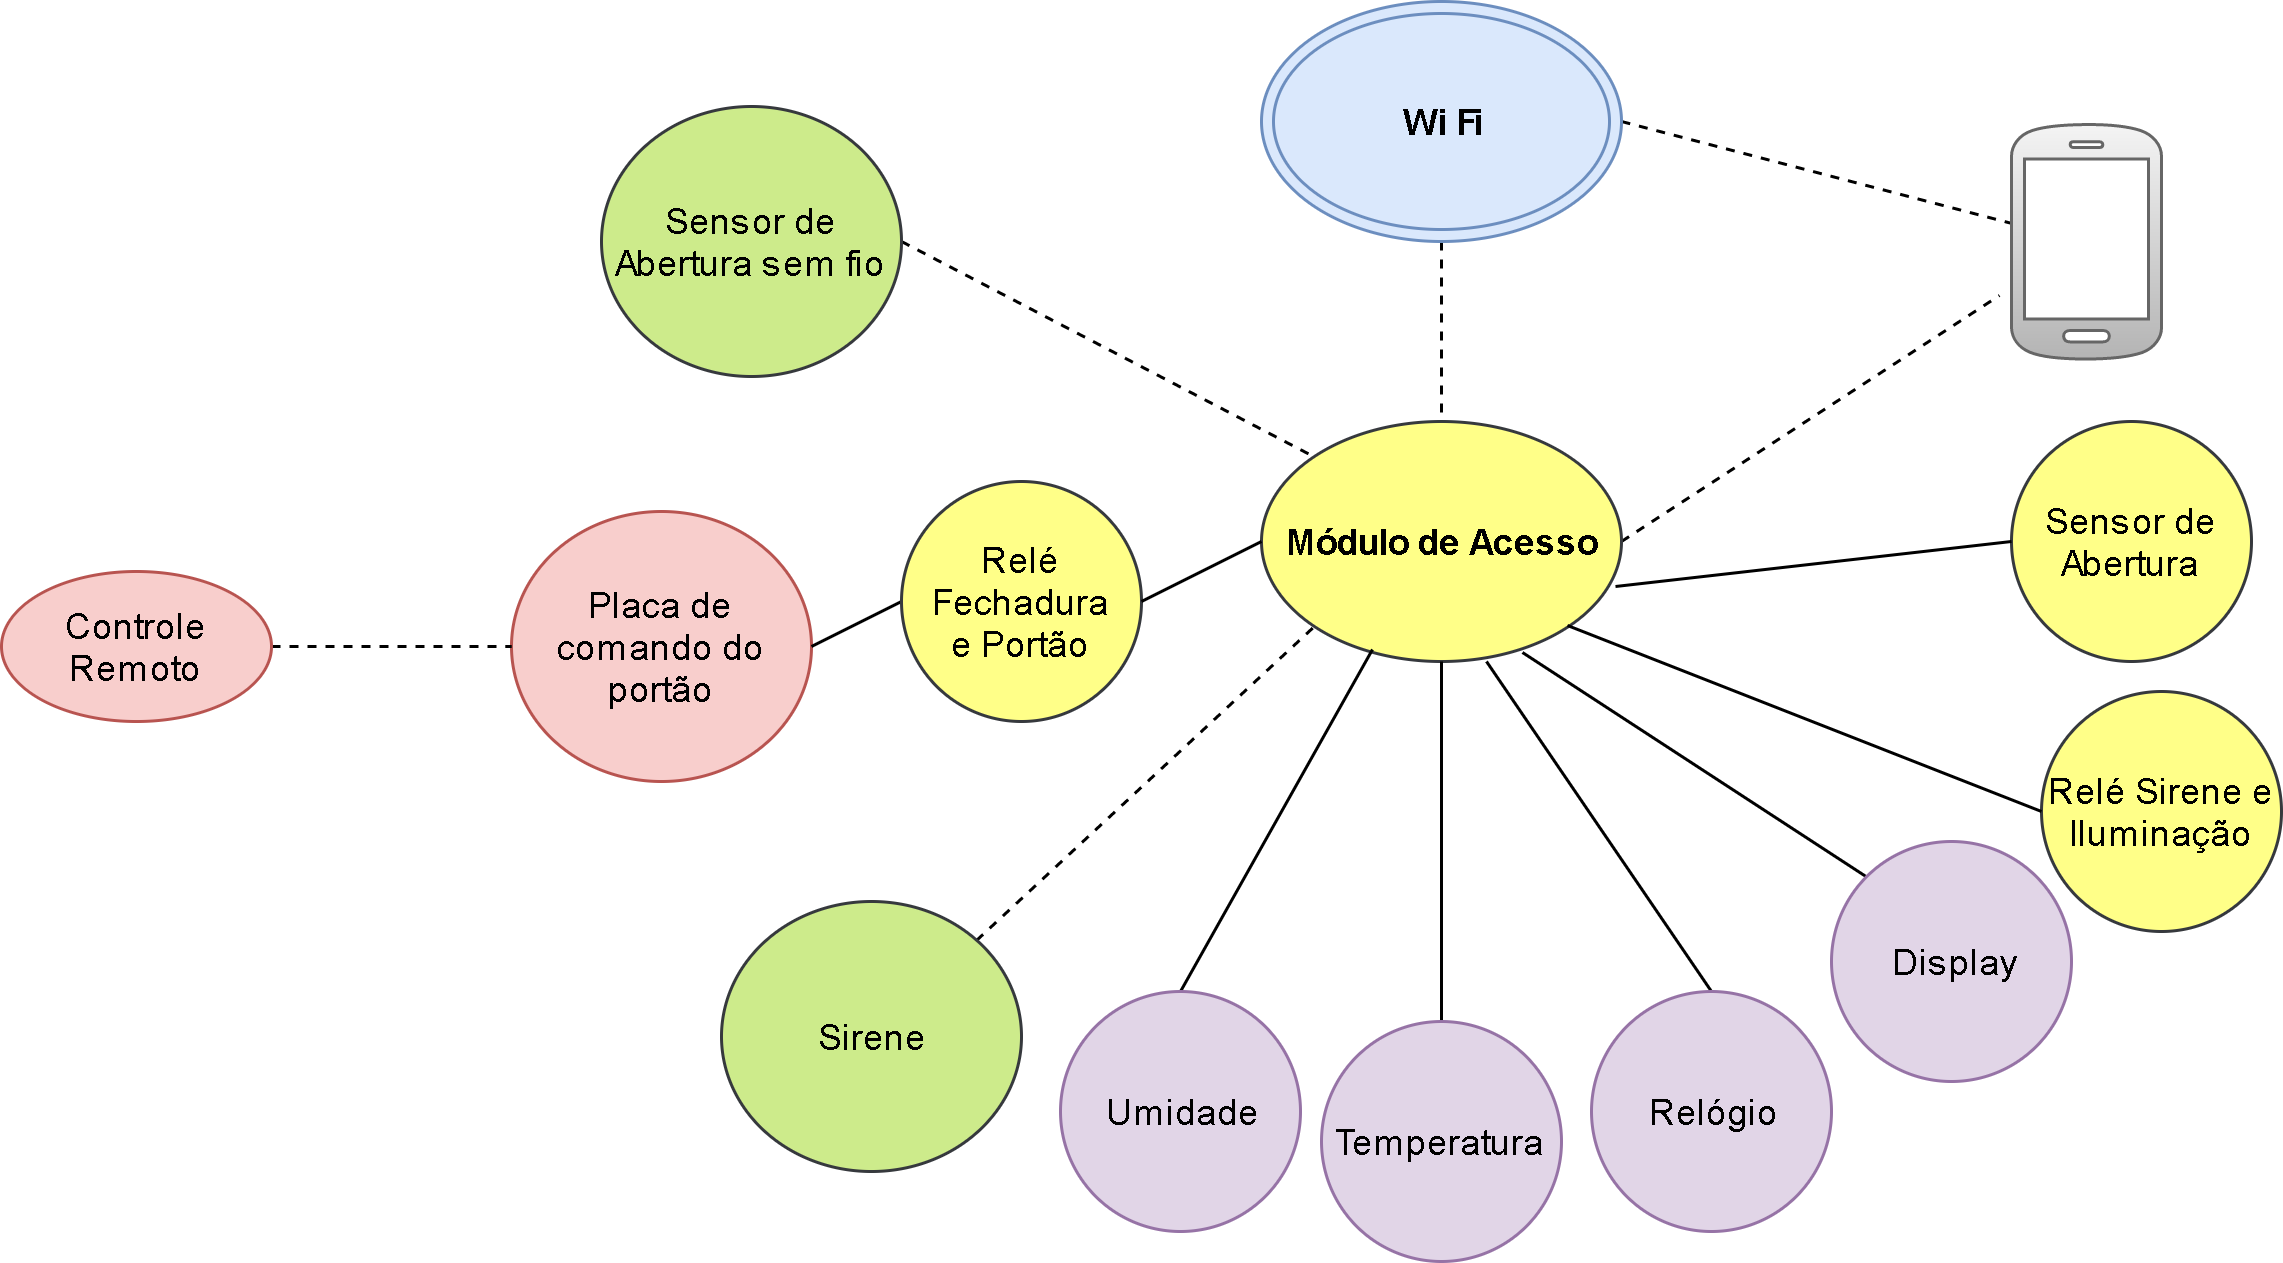
\includegraphics[width=0.8\textwidth]{diagramaModuloAcesso}
\label{fig:diagramaModuloAcesso}
\end{figure}

O diagrama ilustra, em vermelho, os sistemas já existentes. Sensor e sirene sem fio adicionais são mostrados em verde (dispositivos externos ao módulo, que se comunicam por rádio); o próprio módulo de acesso, com um buzzer embutido, e sua conexão com a rede local Wi-Fi ou sua conexão direta com o celular (quando o módulo opera como um ponto de acesso de rede) em amarelo, além de funcionalidades adicionais, em roxo.

A comodidade, no exemplo em questão, está em abrir o portão por meio do celular, ao utilizar o aplicativo web ou o aplicativo local (de emergência), sem a necessidade de carregar uma chave ou controle.

Entretanto, é necessário realizar que a realização do controle de acesso seja feita de maneira segura. Assim, a funcionalidade é apenas local (o usuário deve estar com o celular conectado à rede da casa para acessar a página local), e um algoritmo de rotação de teclas é utilizado, para evitar que pessoas mal intencionadas possam (1) olhar e copiar a senha que o usuário digita em seu celular e (2) copiar os dados de abertura e usá-los mais tarde (“middle man”). Na última alternativa, a cada acesso de um usuário, um novo mapeamento de teclas é gerado e enviado ao usuário. Mesmo que haja cópia, ela não funcionará devido ao mapeamento ter mudado. Observe ainda que a fechadura eletrônica, por si só, já estava vulnerável a este tipo de ataque (há, inclusive, dispositivos copiadores de senhas).

Outro aspecto de segurança é a preocupação dos usuários em esquecer a porta, ou portão, abertos. Para mitigar esse perigo, o módulo deve monitorar, por meio de um sensor, o estado da vigente (aberto/fechado), e alertar localmente (por meio de “buzzer”) e remotamente (e.g. por email ou notificação no \textit{smartphone}) o usuário. Essa e outras configurações (como de rede) são acessadas por uma senha diferente daquela de abertura, de modo que a interface básica seja simples para uso.

Para o caso de falha de envio de notificação (e.g. servidor fora do ar, ou indisponibilidade na conexão), há um algoritmo de novas tentativas com tempos progressivamente maiores conforme as falhas ocorrerem, buscando deixar o módulo disponível para outras funções. Tratamento análogo é realizado no servidor local, e no sistema de mensageria, de modo a evitar perdas de mensagens, mesmo em situações desfavoráveis. Para o caso de falta de conexão à internet, o módulo não seria controlável pela nuvem, com o aplicativo web, mas sim com o aplicativo emergencial, com a ativação do \textit{Access Point}, desenvolvido para operar diretamente com os módulos, sem intermédio do servidor local e dos serviços remotos.

% TODO (victor) checar esse parágrafo abaixo. Acho que não ficou claro o que é esse "travamento"
Para garantir que o módulo está ativo, utiliza-se um sinal de “keep alive” monitorado, e um circuito anti-travamento deve ativar um “hard reset” (reset por hardware), ou então uma rotina de “soft reset” deve ser acionada. No entanto, observe que a segunda alternativa é a mais fácil de implementar, mas é menos robusta, já que ainda pode não funcionar em casos de loop infinito.

% TODO (victor) não entendi a parte do "executa algoritmo análogo ao do envio de emails"
Outra situação que poderia gerar indisponibilidade do sistema é um ataque de DoS local (“Evil Twin”), no qual uma rede mal intencionada usa o mesmo SSID (\textit{Service Set Identifier}, o nome associado à rede WLAN) da rede original, tentando obter a senha na ocasião de reconexão de módulos. Muitas vezes, é também acompanhado de rádio interferência e outros procedimentos para fazer os módulos se desconectarem. Para mitigar o risco, cada módulo tenta inicialmente se conectar usando uma senha falsa no SSID fornecido. Caso obtenha sucesso (se a rede for aberta, como é o caso na maioria desses ataques), ele executa algoritmo análogo ao envio de emails (observe que enquanto não está conectado à rede o módulo atua como ponto de acesso e disponibiliza funcionalidades básicas). Caso ele não obtenha sucesso usando a senha errada (portanto, não detectou a situação de “Evil Twin”), o módulo envia a senha correta. Para proteger a rede, um controlador local do sistema pode atuar junto ao roteador e desligar a conexão sem fio enquanto a situação se mantiver.

O controle de acesso pode ser implementado por meio de persistência de dados de login e senha, e o uso de diversas senhas para uma residência (uma para cada morador - isso torna possível o conhecimento dos usuários que abriram o portão sem a necessidade de login prévio, facilitando o uso). O log destes acessos pode ser analisado (utilizando técnicas de Machine Learning) para determinar perfis de acesso, e evoluir até o sistema saber quando houver um acesso em horário inesperado e notificar o usuário remotamente. O aprendizado de máquina é fundamental aqui para descobrir comportamentos que podem ser entendidos como suspeitos. Para um usuário que costuma chegar em um horário aproximado todos os dias, e acionar funções semelhantes da casa, uma tentativa de acesso que não se enquadre em tais padrões pode ser produto de atividade criminosa, a qual pode ser informada pela casa para uma central, que acionará a polícia caso não seja um falso positivo.
